\begin{center}
    {\LARGE \textbf{2026有机化学与分析化学}} \\[2ex]
    {\large 时量180分钟 \quad 满分150分}
\end{center}

\vspace{0.5cm}
\noindent\textbf{注意事项:}
\begin{enumerate}[label=\arabic*., parsep=0pt, itemsep=0pt]
    \item 答题前,考生先将自己的姓名、学号、考场号、座位号填写在答题卡上,将条形码准确粘贴在考生信息条形码粘贴区。
    \item 考试结束后,将本试卷与答题纸一并收回。
    \item 回答各个问题时,将答案写在答题纸上,写在本试卷上无效。
\end{enumerate}

\vspace{1cm}
\begin{center}
    {\Large \textbf{有机化学部分(共100分)}}
\end{center}

\vspace{0.5cm}
\noindent\textbf{一、选择题(15 pts.)}

\begin{enumerate}[label=\arabic*., itemsep=1.5ex]
    \item (R)-丁-2-醇反应得到(S)-2-溴丁烷的反应机理是
    \begin{tasks}(4)
        \task $S_N1$
        \task E1
        \task E2
        \task $S_N2$
    \end{tasks}
    \item 下列化合物中，酸性最强的是
    \begin{tasks}(4)
        \task \ce{MeOCH2COOH}
        \task \ce{CH3CH2COOH}
        \task \ce{Cl3CCOOH}
        \task \ce{ClCH2COOH}
    \end{tasks}
    \item 下列化合物中，硝化反应速率最快的是
    \begin{tasks}(4)
        \task 甲苯
        \task 硝基苯
        \task 吡啶
        \task 噻吩
    \end{tasks}
    \item 喹啉的亲电取代反应优先进入的位点是
    \begin{center}
        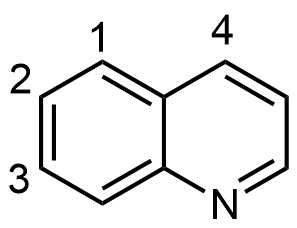
\includegraphics[scale=0.38, valign=c]{./Figure/2026/2026_4_4.png}
    \end{center}
    \begin{tasks}(4)
        \task 1
        \task 2
        \task 3
        \task 4
    \end{tasks}
    \item 苄基甲基醚对下列哪个试剂不稳定
    \begin{tasks}(4)
        \task 丁基锂
        \task Grignard试剂
        \task 碱
        \task 酸
    \end{tasks}
    \item 如下化合物中，酸性最强的氢位于哪个碳上
    
    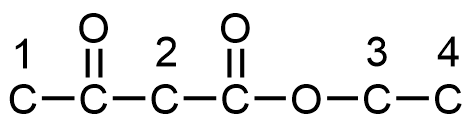
\includegraphics[scale=0.38, valign=c]{./Figure/2026/2026_4_6.png} 
    \begin{tasks}(4)
        \task 1
        \task 2
        \task 3
        \task 4
    \end{tasks}
    \item 下列共轭烯烃中，不能作为双烯体与乙烯发生[4+2]环加成的是
    
    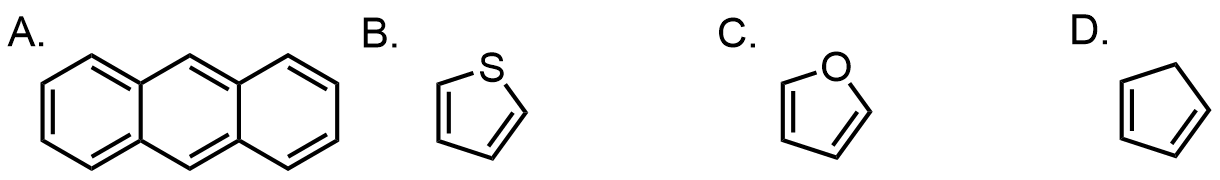
\includegraphics[scale=0.38, valign=c]{./Figure/2026/2026_4_7.png} 
    \item 下列极限共振式中，对共轭体系贡献最大的是
    
    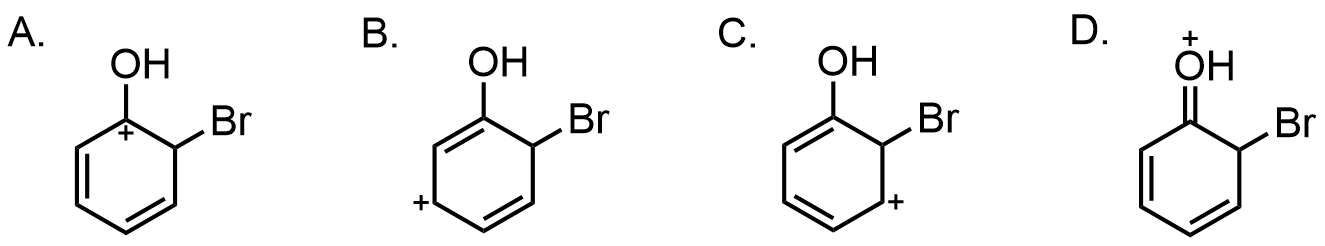
\includegraphics[scale=0.38, valign=c]{./Figure/2026/2026_4_8.png} 
    \item 下列化合物不具有芳香性的是
    
    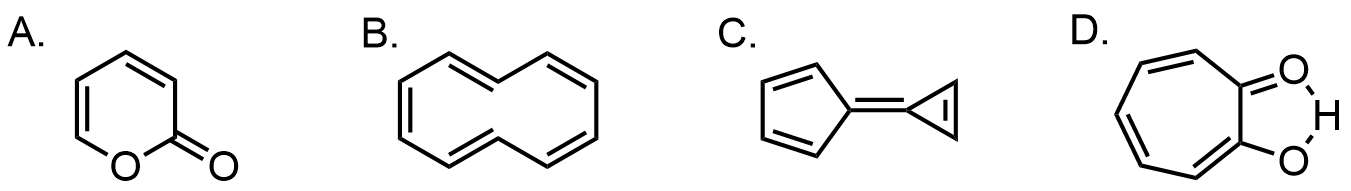
\includegraphics[scale=0.38, valign=c]{./Figure/2026/2026_4_9.png}
    \item 下列化合物中，烯醇式含量最高的是
    \begin{tasks}(2)
        \task \ce{CH3COCH2CHO}
        \task \ce{CH3COCH2COCH3}
        \task \ce{CH2(COOEt)2}
        \task \ce{CH3COCH2COOEt}
    \end{tasks}
    \item 如下反应的产物是
    
    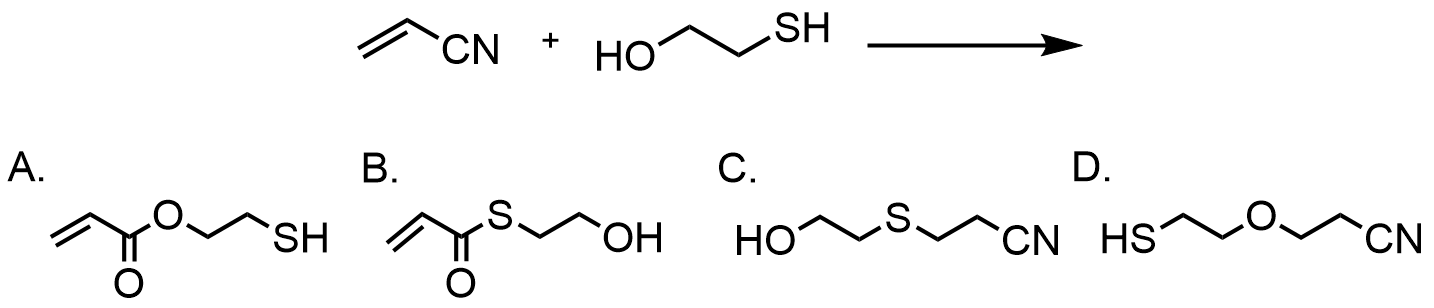
\includegraphics[scale=0.38, valign=c]{./Figure/2026/2026_4_11.png}
    \item 下列化合物中，不具有手性的分子是
    
    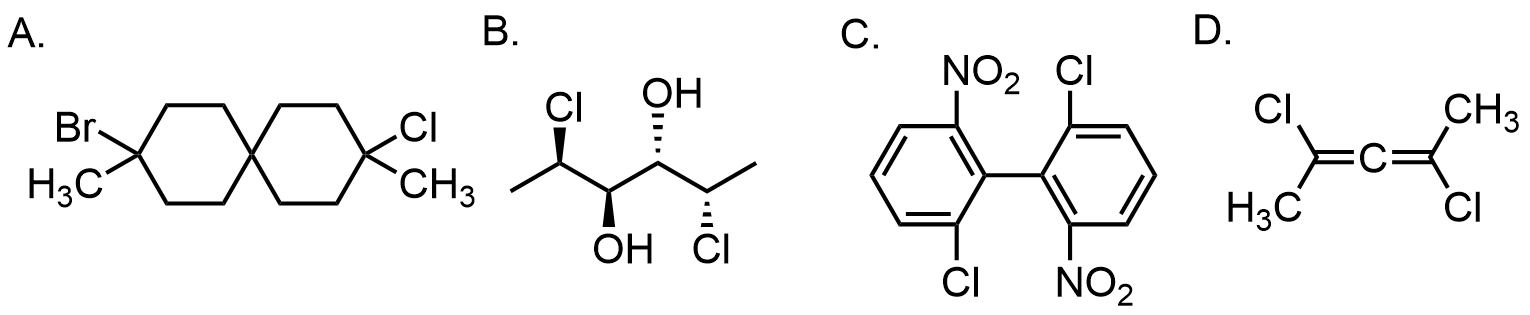
\includegraphics[scale=0.38, valign=c]{./Figure/2026/2026_4_12.png}
    \item 将化合物Q加热到200℃，主产物是
    
    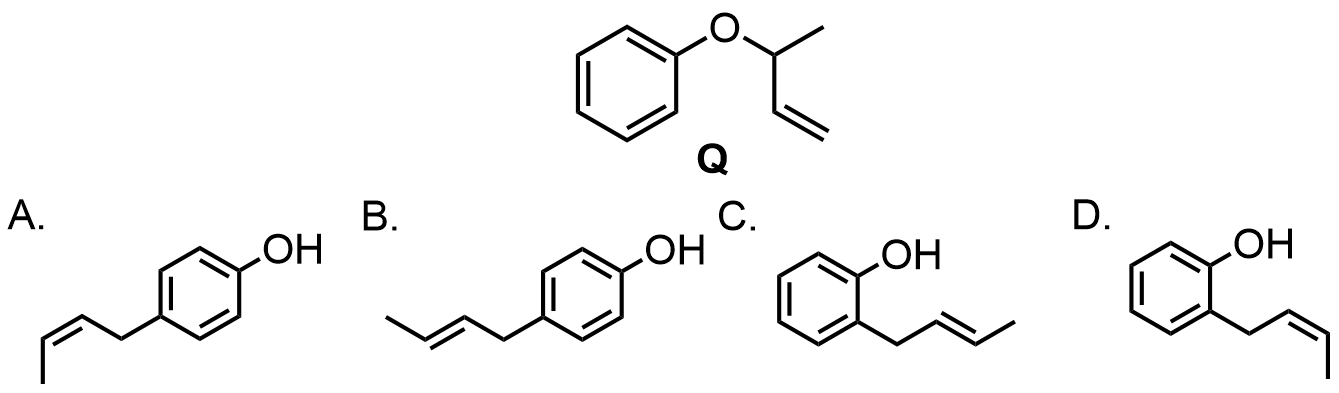
\includegraphics[scale=0.38, valign=c]{./Figure/2026/2026_4_13.png}
    \item 3-甲基环己烯于NBS/ROOR反应条件下在CCl4中回流，主产物是：
    
    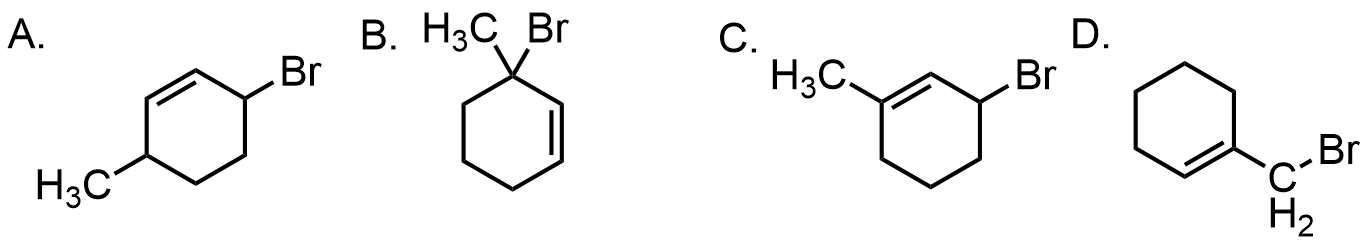
\includegraphics[scale=0.38, valign=c]{./Figure/2026/2026_4_14.png}
    \item 用\ce{NaNH2}/\ce{NH3}(l)处理1-甲氧基-2-氯苯得到
    
    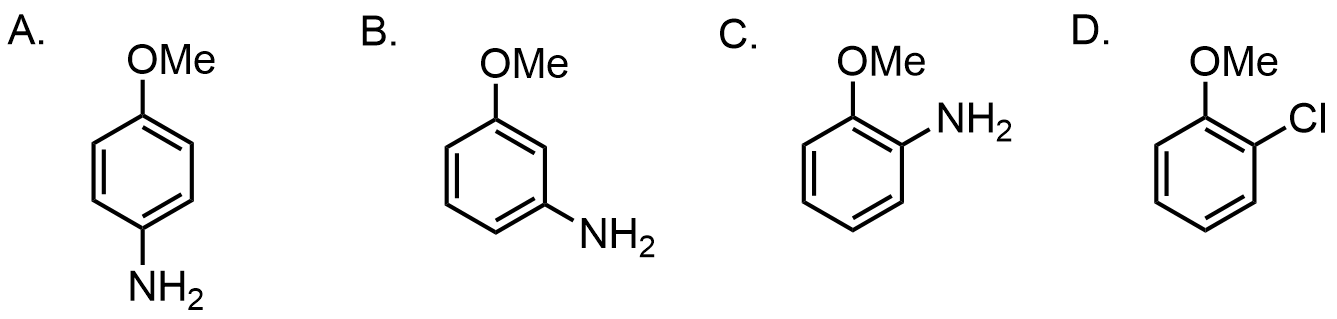
\includegraphics[scale=0.38, valign=c]{./Figure/2026/2026_4_15.png}
\end{enumerate}

\vspace{0.5cm}
\noindent\textbf{二、完成反应(25 pts.)}

\begin{enumerate}[label=\arabic*., itemsep=3ex]
    \item 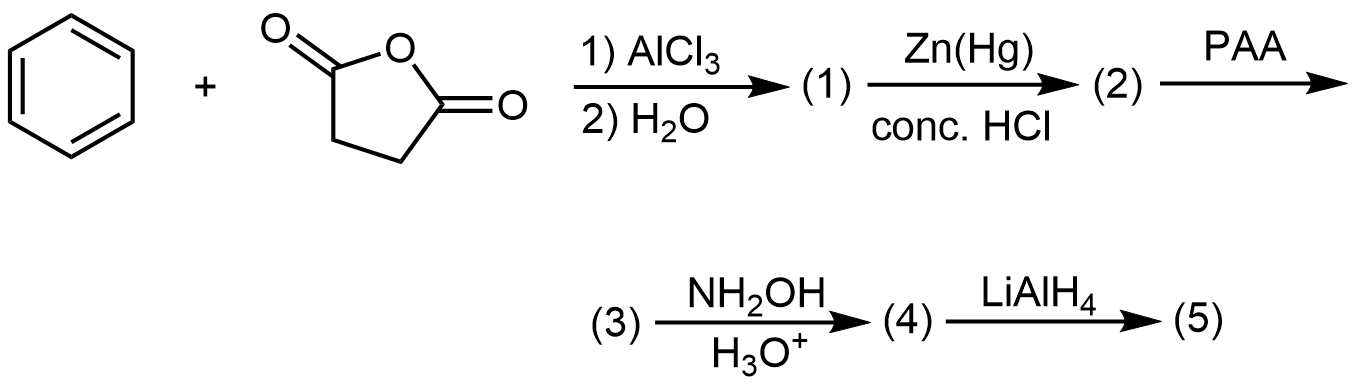
\includegraphics[scale=0.3, valign=c]{./Figure/2026/2026_1_1.png} 
    \item 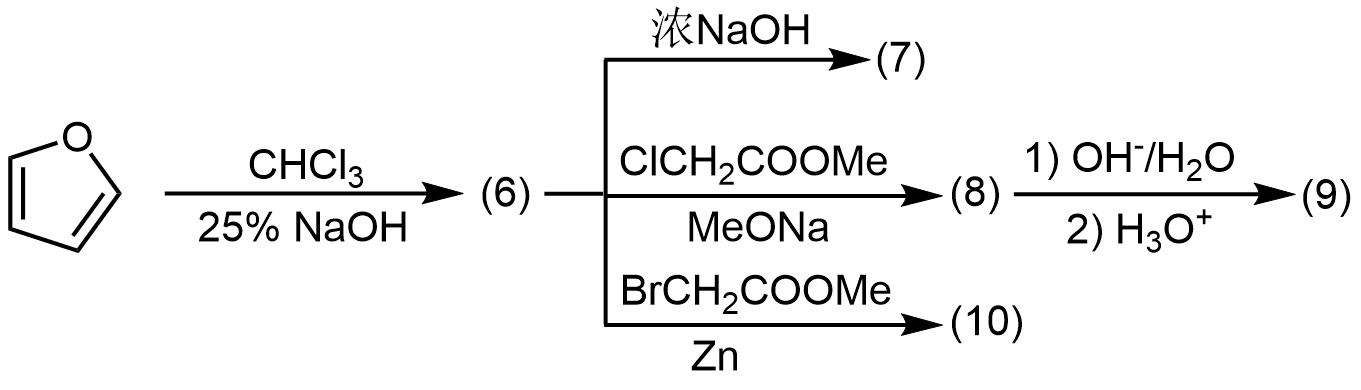
\includegraphics[scale=0.3, valign=c]{./Figure/2026/2026_1_2.png}
    \item 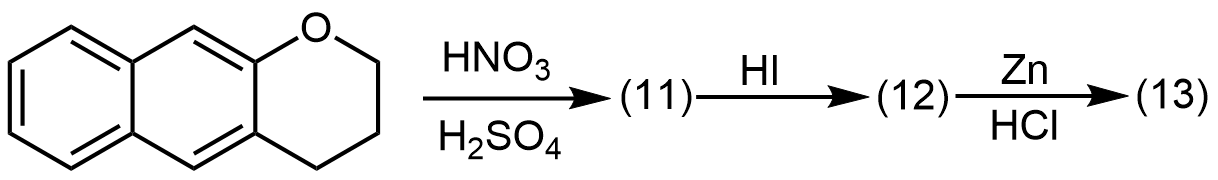
\includegraphics[scale=0.3, valign=c]{./Figure/2026/2026_1_3.png}
    \item 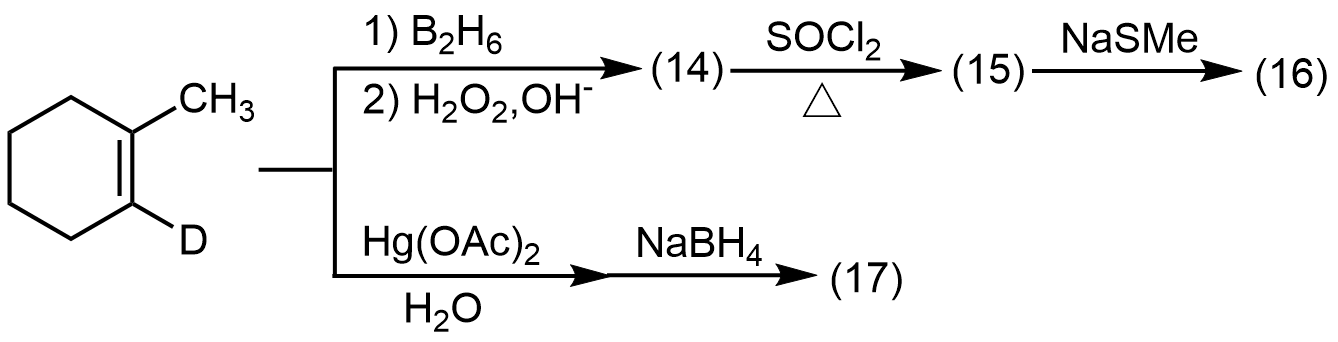
\includegraphics[scale=0.3, valign=c]{./Figure/2026/2026_1_4.png}
    \item 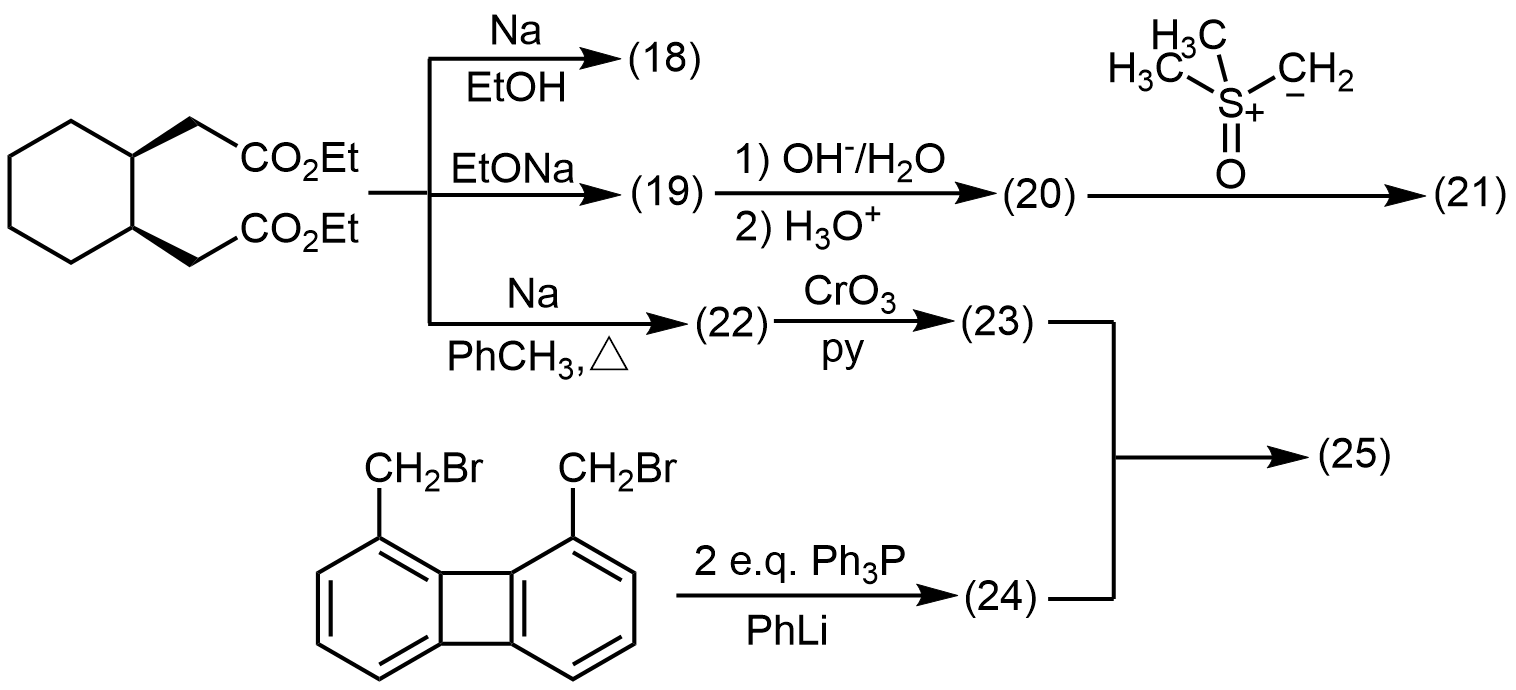
\includegraphics[scale=0.3, valign=c]{./Figure/2026/2026_1_5.png}

\end{enumerate}

\vspace{0.5cm}
\noindent\textbf{三、简答题(12 pts.)}

\begin{enumerate}[label=\arabic*., itemsep=3ex]
    \item 解释吡啶亲电取代取代优先发生在3位、亲核取代优先发生在2、4位的原因
    \begin{center}
        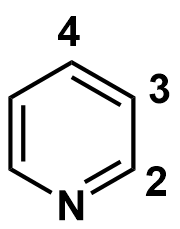
\includegraphics[scale=0.3, valign=c]{./Figure/2026/2026_5_1.png}
    \end{center}
    \item 设计如下过程合成A，但未成功，实际发生下方反应得到了B。从目标分子的结构和反应机理两个角度论述原因。
    \begin{center}
        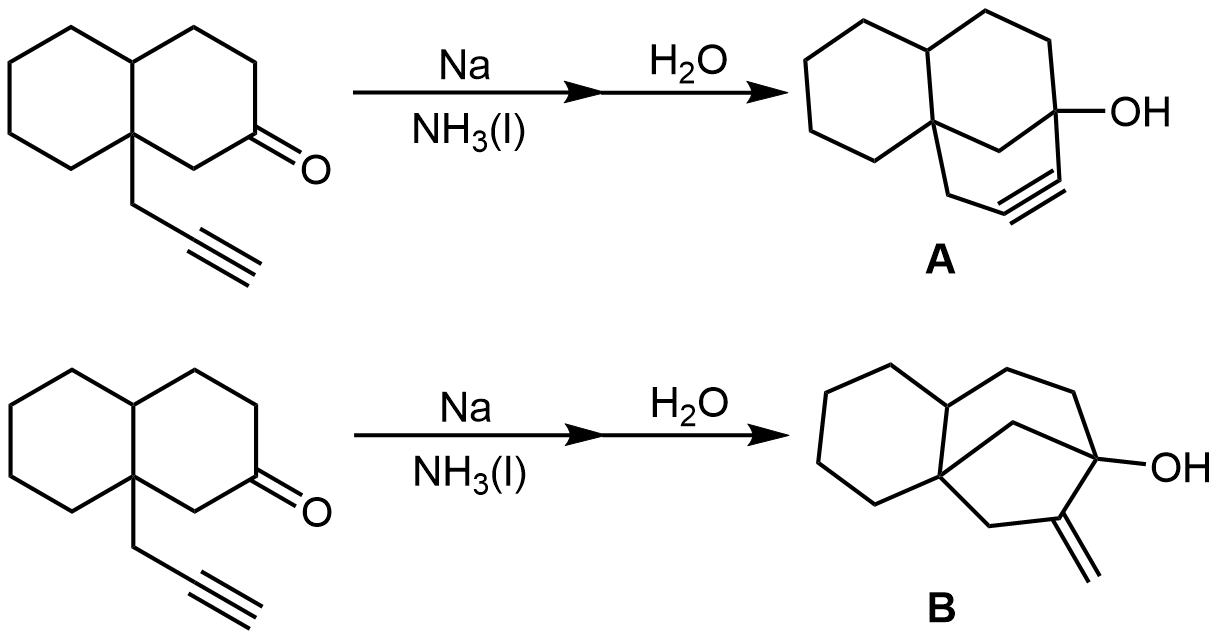
\includegraphics[scale=0.3, valign=c]{./Figure/2026/2026_5_2.png}
    \end{center}
\end{enumerate}


\vspace{0.5cm}
\noindent\textbf{四、机理题(18 pts.)}

\begin{enumerate}[label=\arabic*., start=1, itemsep=1.5ex]
    \item 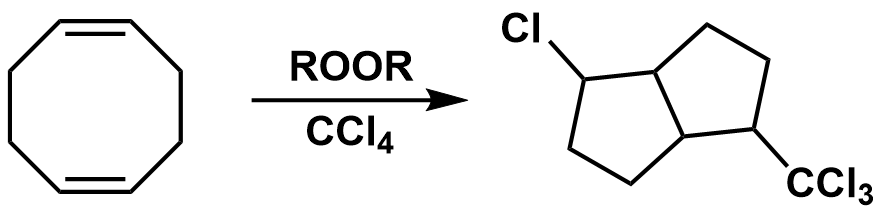
\includegraphics[scale=0.3, valign=c]{./Figure/2026/2026_2_1.png}
    \item 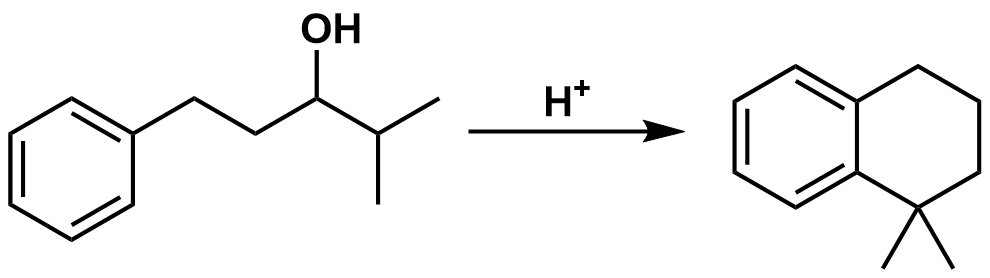
\includegraphics[scale=0.3, valign=c]{./Figure/2026/2026_2_2.png}
    \item 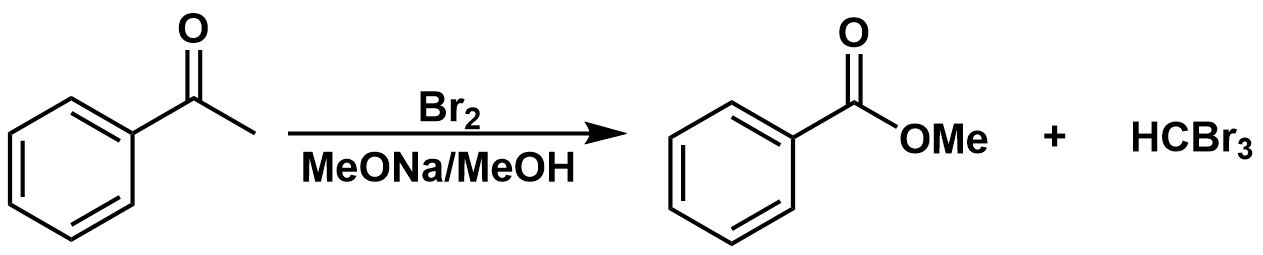
\includegraphics[scale=0.3, valign=c]{./Figure/2026/2026_2_3.png}
\end{enumerate}

\vspace{0.5cm}
\noindent\textbf{五、合成题(30 pts.)}

\begin{enumerate}[label=\arabic*., start=1, itemsep=1.5ex]

    \begin{figure}[htbp]
        \centering
        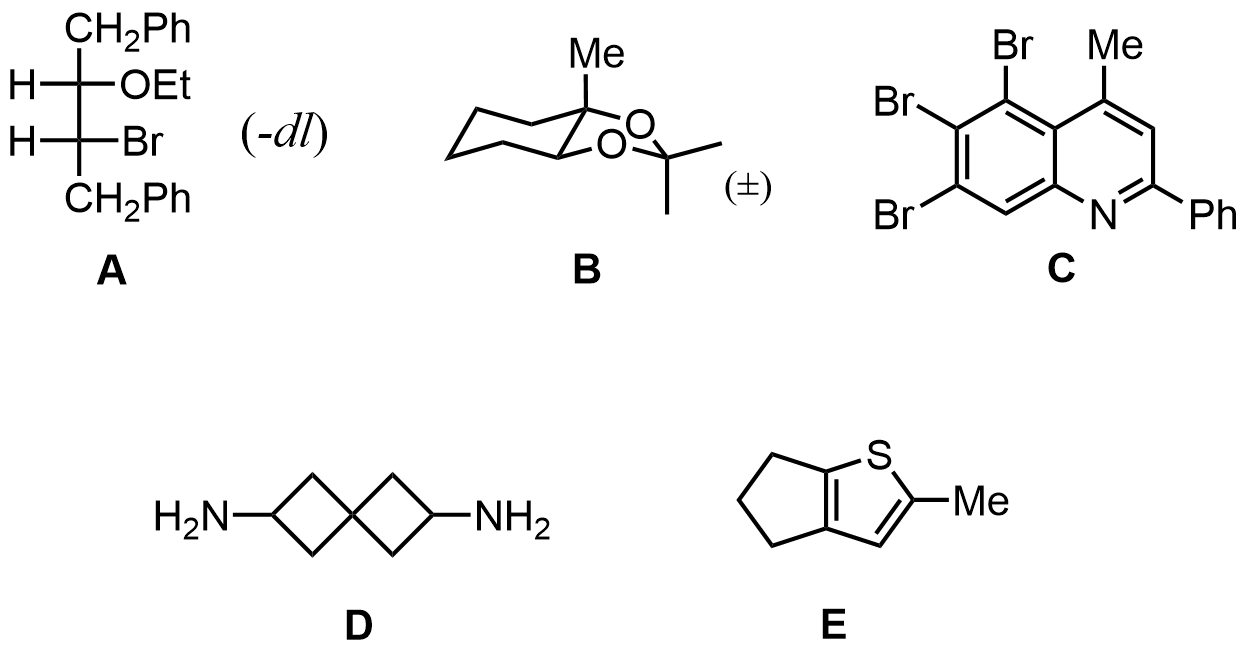
\includegraphics[scale=0.38]{./Figure/2026/2026_3.png}
    \end{figure}
    \item 以苯、小于等于2个碳的有机物合成\textbf{A}
    \item 以小于等于3个碳的有机物合成\textbf{B}
    \item 以苯或甲苯、小于等于3个碳的有机物合成\textbf{C}
    \item 以小于等于3个碳的有机物合成\textbf{D}
    \item 以环戊醇、小于等于2个碳的有机物合成\textbf{E}
\end{enumerate}

\vspace{1cm}
\begin{center}
    {\Large \textbf{分析化学部分(共50分)}}
\end{center}


\vspace{0.5cm}
\noindent\textbf{六、选择题(20 pts.)}

\begin{enumerate}[label=\arabic*., itemsep=1.5ex]
    \item 以某吸附指示剂($\text{p}K_a=5.0$)作为银量法的指示剂，测定的pH应控制在
    \begin{tasks}(4)
        \task $\text{pH}<5.0$
        \task $\text{pH}>5.0$
        \task $5.0<\text{pH}<10.0$
        \task $\text{pH}>10.0$
    \end{tasks}

    \item 有两组分析数据，若要比较他们的精密度有无显著性差异，则应当用
    \begin{tasks}(4)
        \task $F$检验
        \task $t$检验
        \task $u$检验
        \task $Q$检验
    \end{tasks}

    \item 含有$0.10\ \mathrm{mol/L}\ \ce{HCl}$和$0.20\ \mathrm{mol/L}\ \ce{H2SO4}$的混合溶液的质子条件式是
    \begin{tasks}(1)
        \task $[\ce{H+}]=[\ce{OH-}]+2[\ce{Cl-}]+[\ce{SO4^{2-}}]$
        \task $[\ce{H+}]+0.3=[\ce{OH-}]+[\ce{SO4^{2-}}]$
        \task $[\ce{H+}]-0.3=[\ce{OH-}]+[\ce{SO4^{2-}}]$
        \task $[\ce{H+}]-0.3=[\ce{OH-}]+[\ce{SO4^{2-}}]+[\ce{HSO4-}]$
    \end{tasks}

    \item EDTA与金属离子络合时，一分子的EDTA可提供的配位原子个数是
    \begin{tasks}(4)
        \task 2
        \task 4
        \task 6
        \task 8
    \end{tasks}

    \item 若络合滴定反应为：$\ce{M + Y = MY}$，则酸效应系数$\alpha_{Y(\text{H})}$的表达式为
    \begin{tasks}(2)
        \task $[\ce{Y}]/c(\ce{Y})$
        \task $\sum[\ce{H_iY}]/c(\ce{Y})$
        \task $[\ce{Y}]/(\sum[\ce{H_iY}]+[\ce{Y}])$
        \task $(\sum[\ce{H_iY}]+[\ce{Y}])/[\ce{Y}]$
    \end{tasks}

    \item 用重量法测定试样中的砷，首先使其形成$\ce{Ag3AsO4}$沉淀，然后转化为$\ce{AgCl}$，并以此为称量形，则用$\ce{As2O3}$表示的换算因数是
    \begin{tasks}(2)
        \task $M(\ce{As2O3})/M(\ce{AgCl})$
        \task $2M(\ce{As2O3})/3M(\ce{AgCl})$
        \task $3M(\ce{AgCl})/M(\ce{As2O3})$
        \task $M(\ce{As2O3})/6M(\ce{AgCl})$
    \end{tasks}

    \item 以下银量法测定需采用返滴定方式的是
    \begin{tasks}(1)
        \task 莫尔法测$\ce{Cl-}$
        \task 吸附指示剂法测$\ce{Cl-}$
        \task 佛尔哈德法测$\ce{Cl-}$
        \task $\ce{AgNO3}$滴定$\ce{CN-}$(生成$\ce{Ag[Ag(CN)2]}$指示终点)
    \end{tasks}

    \item 为了消除$0.001000\ \mathrm{kg}$中的非有效数字，将该数值正确地表示为以克(g)为单位的数值结果为
    \begin{tasks}(4)
        \task $1\ \mathrm{g}$
        \task $1.0\ \mathrm{g}$
        \task $1.00\ \mathrm{g}$
        \task $1.000\ \mathrm{g}$
    \end{tasks}

    \item $\ce{Fe^{3+}}$与$\ce{Sn^{2+}}$反应的平衡常数对数值为
    \\
    已知：$\varphi^\ominus(\ce{Fe^{3+}/Fe^{2+}})=0.77\ \mathrm{V}$，$\varphi^\ominus(\ce{Sn^{4+}/Sn^{2+}})=0.15\ \mathrm{V}$
    \begin{tasks}(2)
        \task $(0.77-0.15)/0.059$
        \task $2\times(0.77-0.15)/0.059$
        \task $3\times(0.77-0.15)/0.059$
        \task $2\times(0.15-0.77)/0.059$
    \end{tasks}

    \item 下列表述中错误的是
    \begin{tasks}(1)
        \task 由于无定形沉淀颗粒小，为防止沉淀穿滤，应选用致密滤纸（慢速）
        \task 微溶化合物的临界值$(Q/S)$愈大，则愈不容易均相成核
        \task 相对过饱和度愈大，分散度愈高
        \task 均相成核作用是指构晶离子自发形成晶核
    \end{tasks}
\end{enumerate}

\vspace{0.5cm}
\noindent\textbf{七、填空题(20 pts.)}

\begin{enumerate}[label=\arabic*., itemsep=1.5ex]
    \item 根据：$\varphi^\ominus(\ce{Fe^{2+}/Fe})=-0.440\ \mathrm{V}$、$\varphi^\ominus(\ce{Sn^{4+}/Sn^{2+}})=0.154\ \mathrm{V}$、$\varphi^\ominus(\ce{Sn^{2+}/Sn})=-0.136\ \mathrm{V}$、$\varphi^\ominus(\ce{Cu^{2+}/Cu^{+}})=0.159\ \mathrm{V}$、$\varphi^\ominus(\ce{Cu^{+}/Cu})=0.522\ \mathrm{V}$，判断在酸性溶液中金属铁还原$\ce{Sn^{4+}}$时生成\underline{\qquad\qquad}，而还原$\ce{Cu^{2+}}$时则生成\underline{\qquad\qquad}。
    \item 若滴定剂与被测物溶液浓度均增加10倍，$\ce{NaOH}$滴定$\ce{HCl}$的滴定突跃\underline{\qquad\qquad}；$\ce{NaOH}$滴定$\ce{HAc}$的滴定突跃\underline{\qquad\qquad}。（指pH增加或减少多少单位）
    \item 用强酸性阳离子交换树脂分离$\ce{Na+}$、$\ce{K+}$、$\ce{Cs+}$、$\ce{Rb+}$、$\ce{Li+}$，以$0.1\ \mathrm{mol/L}$的$\ce{HCl}$溶液洗脱，各个离子流出色谱柱的先后顺序为\underline{\qquad\qquad}。
    \item $\ce{Fe^{3+}/Fe^{2+}}$电对电位在加入$\ce{HCl}$后会\underline{\qquad\qquad}；加入邻二氮菲后会\underline{\qquad\qquad}。（填“增加”、“降低”或“不变”）
    \item 实验证明，在较低浓度$\ce{Na2SO4}$存在下，相比纯水$\ce{PbSO4}$的溶解度降低；但当$\ce{Na2SO4}$的浓度$c\ge0.2\ \mathrm{mol\cdot L^{-1}}$时，$\ce{PbSO4}$的溶解度却增大，这是因为\underline{\qquad\qquad}。
    \item 在弱碱性溶液中用EDTA滴定$\ce{Zn^{2+}}$，常使用$\ce{NH3-NH4+}$溶液，其作用是\underline{\qquad\qquad}、\underline{\qquad\qquad}。
    \item $\ce{H3PO4}$的 $\text{p}K_{a1}=2.12$，$\text{p}K_{a2}=7.20$，$\text{p}K_{a3}=12.36$，则$\ce{PO4^{3-}}$的 $\text{p}K_{b1}=$\underline{\qquad\qquad}，$\text{p}K_{b2}=$\underline{\qquad\qquad}。
    \item EDTA滴定金属M的离子的过程中，介质pH越低，则$\alpha_{Y(\text{H})}$值越\underline{\qquad\qquad}，$K'_{\text{MY}}$值越\underline{\qquad\qquad}。（填“大”或“小”）
    \item 某人误将参比溶液的透射比调至98\%，而不是100\%，在此条件下测得有色溶液的透射比为36\%，则该有色溶液的正确透射比应为\underline{\qquad\qquad}。
    \item 已知EDTA($\ce{H6Y^{2+}}$)的 $\text{p}K_{a1}\sim\text{p}K_{a6}$分别为0.9、1.6、2.0、2.67、6.16、10.26，在$\text{pH}<1.0$的溶液中，EDTA的主要存在形式是\underline{\qquad\qquad}；$\text{pH}=5.0$时是\underline{\qquad\qquad}。
\end{enumerate}

\vspace{0.5cm}
\noindent\textbf{八、解答题(10 pts.)}
用某分析方法测定某试样中$\ce{Fe2O3}$的质量分数，重复测定6次，结果分别为：41.0\%、42.0\%、43.0\%、44.0\%、43.0\%、43.0\%。
\begin{enumerate}[label=(\arabic*), itemsep=1.5ex]
    \item 在90\%置信水平下，采用$Q$检验法判断是否存在可疑值；
    \item 根据(1)的判断结果，计算$\ce{Fe2O3}$质量分数的平均值(保留三位有效数字)；
    \item 采用标准方法测得该试样$\ce{Fe2O3}$质量分数为40.0\%，该标准方法的标准偏差为$s=1.03\%$。在95\%置信水平下，判断本方法结果是否存在系统误差。
\end{enumerate}

已知：$Q_{0.10,5}=0.64$，$Q_{0.10,6}=0.56$，$Q_{0.10,7}=0.51$

$t_{0.05,5}=2.57$，$t_{0.05,6}=2.45$，$t_{0.10,5}=2.02$，$t_{0.10,6}=1.94$